\section{Mini-mundo: números racionales}

El modelo original del equipo, reproducido en la
Figura~\ref{fig:numeros-racionales}, representa cada fracción mediante la
entidad \textbf{NúmeroRacional}. Los atributos subrayados \emph{Numerador} y
\emph{Denominador} forman conjuntamente su identificador. Por ello, dos
fracciones se consideran distintas cuando cambia cualquiera de ambos valores,
aunque su forma simplificada sea la misma. El denominador debe ser distinto de
cero.

\begin{figure}[htbp]
  \centering
  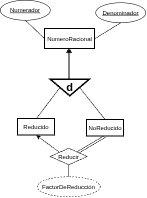
\includegraphics[height=0.58\textheight]{../Diagramas/Ejercicio3a.drawio.png}
  \caption{Modelo E--R original para números racionales.}
  \label{fig:numeros-racionales}
\end{figure}

La especialización total y disjunta divide a \textbf{NúmeroRacional} en
\textbf{Reducido} y \textbf{NoReducido}. El símbolo ``d'' expresa que una
instancia sólo puede pertenecer a uno de esos subtipos, mientras la conexión
doble con la superentidad indica que todo número racional se clasifica en uno
de ellos.

La relación \textbf{Reducir} vincula una fracción no reducida con su fracción
reducida. La dirección de las flechas expresa la unicidad representada por el
equipo: cada fracción no reducida posee una sola forma totalmente simplificada.
El atributo \emph{FactorDeReducción} pertenece a esta relación porque depende
de la pareja formada por ambas fracciones; su óvalo discontinuo indica que se
considera derivable a partir de sus numeradores y denominadores.

Para cada reducción se cumple que el numerador y el denominador originales son
el producto del factor por los valores de la fracción reducida. Asimismo, la
fracción clasificada como \textbf{Reducido} debe tener numerador y denominador
coprimos. Como convención, el signo se mantiene en el numerador y el
denominador reducido es positivo.
